\documentclass[tikz, border=1mm]{standalone}
\begin{document}
\begin{minipage}{\textwidth}
\centering
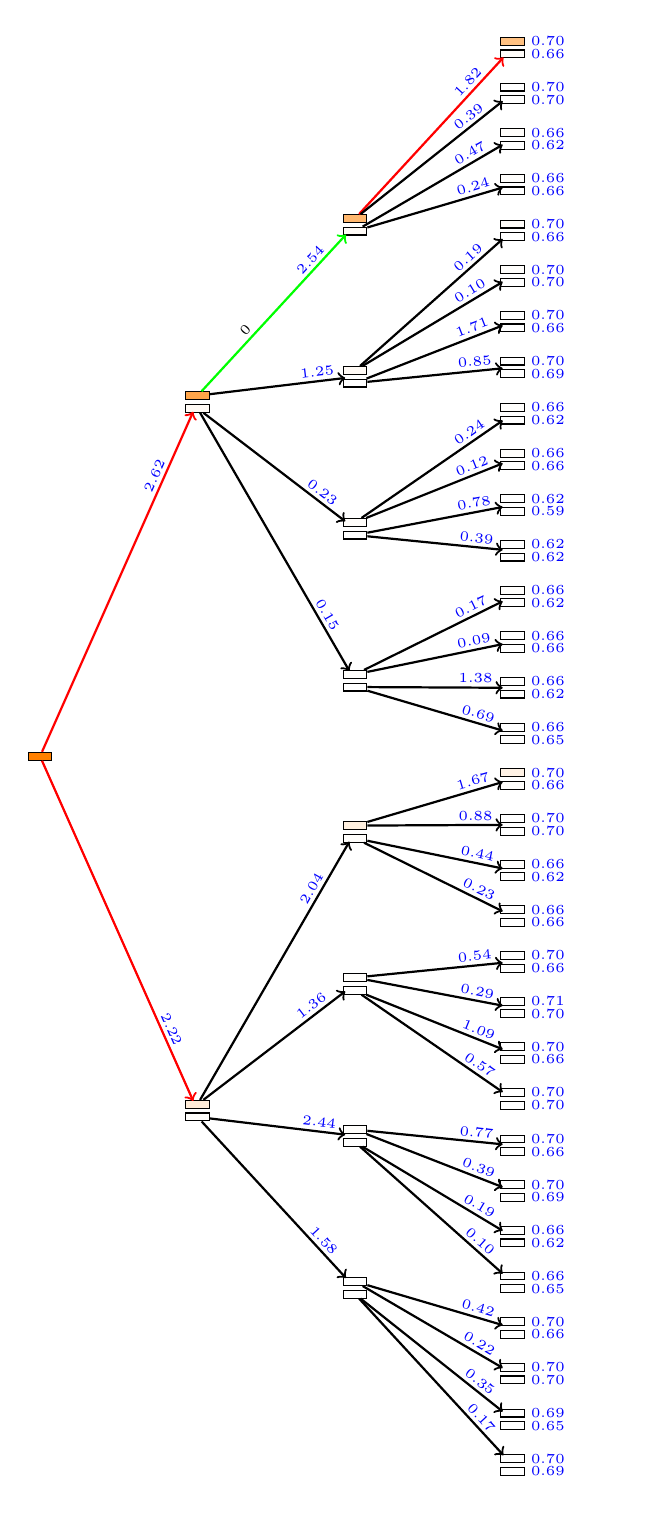
\begin{tikzpicture}
\tikzstyle{between} = [rectangle, draw=none]
\tikzstyle{qval}    = [rectangle, text centered, text width=2cm]
\node[between] at (-8.00, 4.50) (1_b_0){};
\node[between] at (-8.00, -4.50) (1_b_1){};
\node[between] at (-6.00, 6.75) (2_b_0){};
\node[between] at (-6.00, 4.82) (2_b_1){};
\node[between] at (-6.00, 2.89) (2_b_2){};
\node[between] at (-6.00, 0.96) (2_b_3){};
\node[between] at (-6.00, -0.96) (2_b_4){};
\node[between] at (-6.00, -2.89) (2_b_5){};
\node[between] at (-6.00, -4.82) (2_b_6){};
\node[between] at (-6.00, -6.75) (2_b_7){};
\node[between] at (-4.00, 9.00) (3_b_0){};
\node[between] at (-4.00, 8.42) (3_b_1){};
\node[between] at (-4.00, 7.84) (3_b_2){};
\node[between] at (-4.00, 7.26) (3_b_3){};
\node[between] at (-4.00, 6.68) (3_b_4){};
\node[between] at (-4.00, 6.10) (3_b_5){};
\node[between] at (-4.00, 5.52) (3_b_6){};
\node[between] at (-4.00, 4.94) (3_b_7){};
\node[between] at (-4.00, 4.35) (3_b_8){};
\node[between] at (-4.00, 3.77) (3_b_9){};
\node[between] at (-4.00, 3.19) (3_b_10){};
\node[between] at (-4.00, 2.61) (3_b_11){};
\node[between] at (-4.00, 2.03) (3_b_12){};
\node[between] at (-4.00, 1.45) (3_b_13){};
\node[between] at (-4.00, 0.87) (3_b_14){};
\node[between] at (-4.00, 0.29) (3_b_15){};
\node[between] at (-4.00, -0.29) (3_b_16){};
\node[between] at (-4.00, -0.87) (3_b_17){};
\node[between] at (-4.00, -1.45) (3_b_18){};
\node[between] at (-4.00, -2.03) (3_b_19){};
\node[between] at (-4.00, -2.61) (3_b_20){};
\node[between] at (-4.00, -3.19) (3_b_21){};
\node[between] at (-4.00, -3.77) (3_b_22){};
\node[between] at (-4.00, -4.35) (3_b_23){};
\node[between] at (-4.00, -4.94) (3_b_24){};
\node[between] at (-4.00, -5.52) (3_b_25){};
\node[between] at (-4.00, -6.10) (3_b_26){};
\node[between] at (-4.00, -6.68) (3_b_27){};
\node[between] at (-4.00, -7.26) (3_b_28){};
\node[between] at (-4.00, -7.84) (3_b_29){};
\node[between] at (-4.00, -8.42) (3_b_30){};
\node[between] at (-4.00, -9.00) (3_b_31){};
\node[rectangle, text centered, draw=black, minimum height=1mm, text width=3mm, inner sep=0pt, fill=orange, fill opacity=1.00, draw opacity=1] at (-10.00, 0.00) (0_s_0){};
\node[rectangle, text centered, draw=black, minimum height=1mm, text width=3mm, inner sep=0pt, fill=orange, fill opacity=0.71, draw opacity=1] at (-8.00, 4.58) (1_s_0) {};
\node[rectangle, text centered, draw=black, minimum height=1mm, text width=3mm, inner sep=0pt, fill=orange, fill opacity=0.04, draw opacity=1] at (-8.00, 4.42) (1_s_1) {};
\node[rectangle, text centered, draw=black, minimum height=1mm, text width=3mm, inner sep=0pt, fill=orange, fill opacity=0.15, draw opacity=1] at (-8.00, -4.42) (1_s_2) {};
\node[rectangle, text centered, draw=black, minimum height=1mm, text width=3mm, inner sep=0pt, fill=orange, fill opacity=0.01, draw opacity=1] at (-8.00, -4.58) (1_s_3) {};
\node[rectangle, text centered, draw=black, minimum height=1mm, text width=3mm, inner sep=0pt, fill=orange, fill opacity=0.57, draw opacity=1] at (-6.00, 6.83) (2_s_0) {};
\node[rectangle, text centered, draw=black, minimum height=1mm, text width=3mm, inner sep=0pt, fill=orange, fill opacity=0.03, draw opacity=1] at (-6.00, 6.67) (2_s_1) {};
\node[rectangle, text centered, draw=black, minimum height=1mm, text width=3mm, inner sep=0pt, fill=orange, fill opacity=0.04, draw opacity=1] at (-6.00, 4.90) (2_s_2) {};
\node[rectangle, text centered, draw=black, minimum height=1mm, text width=3mm, inner sep=0pt, fill=orange, fill opacity=0.00, draw opacity=1] at (-6.00, 4.74) (2_s_3) {};
\node[rectangle, text centered, draw=black, minimum height=1mm, text width=3mm, inner sep=0pt, fill=orange, fill opacity=0.02, draw opacity=1] at (-6.00, 2.97) (2_s_4) {};
\node[rectangle, text centered, draw=black, minimum height=1mm, text width=3mm, inner sep=0pt, fill=orange, fill opacity=0.00, draw opacity=1] at (-6.00, 2.81) (2_s_5) {};
\node[rectangle, text centered, draw=black, minimum height=1mm, text width=3mm, inner sep=0pt, fill=orange, fill opacity=0.01, draw opacity=1] at (-6.00, 1.04) (2_s_6) {};
\node[rectangle, text centered, draw=black, minimum height=1mm, text width=3mm, inner sep=0pt, fill=orange, fill opacity=0.00, draw opacity=1] at (-6.00, 0.88) (2_s_7) {};
\node[rectangle, text centered, draw=black, minimum height=1mm, text width=3mm, inner sep=0pt, fill=orange, fill opacity=0.12, draw opacity=1] at (-6.00, -0.88) (2_s_8) {};
\node[rectangle, text centered, draw=black, minimum height=1mm, text width=3mm, inner sep=0pt, fill=orange, fill opacity=0.01, draw opacity=1] at (-6.00, -1.04) (2_s_9) {};
\node[rectangle, text centered, draw=black, minimum height=1mm, text width=3mm, inner sep=0pt, fill=orange, fill opacity=0.01, draw opacity=1] at (-6.00, -2.81) (2_s_10) {};
\node[rectangle, text centered, draw=black, minimum height=1mm, text width=3mm, inner sep=0pt, fill=orange, fill opacity=0.00, draw opacity=1] at (-6.00, -2.97) (2_s_11) {};
\node[rectangle, text centered, draw=black, minimum height=1mm, text width=3mm, inner sep=0pt, fill=orange, fill opacity=0.01, draw opacity=1] at (-6.00, -4.74) (2_s_12) {};
\node[rectangle, text centered, draw=black, minimum height=1mm, text width=3mm, inner sep=0pt, fill=orange, fill opacity=0.00, draw opacity=1] at (-6.00, -4.90) (2_s_13) {};
\node[rectangle, text centered, draw=black, minimum height=1mm, text width=3mm, inner sep=0pt, fill=orange, fill opacity=0.00, draw opacity=1] at (-6.00, -6.67) (2_s_14) {};
\node[rectangle, text centered, draw=black, minimum height=1mm, text width=3mm, inner sep=0pt, fill=orange, fill opacity=0.00, draw opacity=1] at (-6.00, -6.83) (2_s_15) {};
\node[rectangle, text centered, draw=black, minimum height=1mm, text width=3mm, inner sep=0pt, fill=orange, fill opacity=0.49, draw opacity=1] at (-4.00, 9.08) (3_s_0) {};
\node[qval] at (-3.55, 9.08) () {\tiny \textcolor{blue}{0.70}};
\node[rectangle, text centered, draw=black, minimum height=1mm, text width=3mm, inner sep=0pt, fill=orange, fill opacity=0.02, draw opacity=1] at (-4.00, 8.92) (3_s_1) {};
\node[qval] at (-3.55, 8.92) () {\tiny \textcolor{blue}{0.66}};
\node[rectangle, text centered, draw=black, minimum height=1mm, text width=3mm, inner sep=0pt, fill=orange, fill opacity=0.00, draw opacity=1] at (-4.00, 8.50) (3_s_2) {};
\node[qval] at (-3.55, 8.50) () {\tiny \textcolor{blue}{0.70}};
\node[rectangle, text centered, draw=black, minimum height=1mm, text width=3mm, inner sep=0pt, fill=orange, fill opacity=0.00, draw opacity=1] at (-4.00, 8.34) (3_s_3) {};
\node[qval] at (-3.55, 8.34) () {\tiny \textcolor{blue}{0.70}};
\node[rectangle, text centered, draw=black, minimum height=1mm, text width=3mm, inner sep=0pt, fill=orange, fill opacity=0.02, draw opacity=1] at (-4.00, 7.92) (3_s_4) {};
\node[qval] at (-3.55, 7.92) () {\tiny \textcolor{blue}{0.66}};
\node[rectangle, text centered, draw=black, minimum height=1mm, text width=3mm, inner sep=0pt, fill=orange, fill opacity=0.00, draw opacity=1] at (-4.00, 7.76) (3_s_5) {};
\node[qval] at (-3.55, 7.76) () {\tiny \textcolor{blue}{0.62}};
\node[rectangle, text centered, draw=black, minimum height=1mm, text width=3mm, inner sep=0pt, fill=orange, fill opacity=0.01, draw opacity=1] at (-4.00, 7.34) (3_s_6) {};
\node[qval] at (-3.55, 7.34) () {\tiny \textcolor{blue}{0.66}};
\node[rectangle, text centered, draw=black, minimum height=1mm, text width=3mm, inner sep=0pt, fill=orange, fill opacity=0.00, draw opacity=1] at (-4.00, 7.18) (3_s_7) {};
\node[qval] at (-3.55, 7.18) () {\tiny \textcolor{blue}{0.66}};
\node[rectangle, text centered, draw=black, minimum height=1mm, text width=3mm, inner sep=0pt, fill=orange, fill opacity=0.02, draw opacity=1] at (-4.00, 6.76) (3_s_8) {};
\node[qval] at (-3.55, 6.76) () {\tiny \textcolor{blue}{0.70}};
\node[rectangle, text centered, draw=black, minimum height=1mm, text width=3mm, inner sep=0pt, fill=orange, fill opacity=0.00, draw opacity=1] at (-4.00, 6.60) (3_s_9) {};
\node[qval] at (-3.55, 6.60) () {\tiny \textcolor{blue}{0.66}};
\node[rectangle, text centered, draw=black, minimum height=1mm, text width=3mm, inner sep=0pt, fill=orange, fill opacity=0.01, draw opacity=1] at (-4.00, 6.18) (3_s_10) {};
\node[qval] at (-3.55, 6.18) () {\tiny \textcolor{blue}{0.70}};
\node[rectangle, text centered, draw=black, minimum height=1mm, text width=3mm, inner sep=0pt, fill=orange, fill opacity=0.00, draw opacity=1] at (-4.00, 6.02) (3_s_11) {};
\node[qval] at (-3.55, 6.02) () {\tiny \textcolor{blue}{0.70}};
\node[rectangle, text centered, draw=black, minimum height=1mm, text width=3mm, inner sep=0pt, fill=orange, fill opacity=0.00, draw opacity=1] at (-4.00, 5.60) (3_s_12) {};
\node[qval] at (-3.55, 5.60) () {\tiny \textcolor{blue}{0.70}};
\node[rectangle, text centered, draw=black, minimum height=1mm, text width=3mm, inner sep=0pt, fill=orange, fill opacity=0.00, draw opacity=1] at (-4.00, 5.44) (3_s_13) {};
\node[qval] at (-3.55, 5.44) () {\tiny \textcolor{blue}{0.66}};
\node[rectangle, text centered, draw=black, minimum height=1mm, text width=3mm, inner sep=0pt, fill=orange, fill opacity=0.00, draw opacity=1] at (-4.00, 5.02) (3_s_14) {};
\node[qval] at (-3.55, 5.02) () {\tiny \textcolor{blue}{0.70}};
\node[rectangle, text centered, draw=black, minimum height=1mm, text width=3mm, inner sep=0pt, fill=orange, fill opacity=0.00, draw opacity=1] at (-4.00, 4.86) (3_s_15) {};
\node[qval] at (-3.55, 4.86) () {\tiny \textcolor{blue}{0.69}};
\node[rectangle, text centered, draw=black, minimum height=1mm, text width=3mm, inner sep=0pt, fill=orange, fill opacity=0.01, draw opacity=1] at (-4.00, 4.43) (3_s_16) {};
\node[qval] at (-3.55, 4.43) () {\tiny \textcolor{blue}{0.66}};
\node[rectangle, text centered, draw=black, minimum height=1mm, text width=3mm, inner sep=0pt, fill=orange, fill opacity=0.00, draw opacity=1] at (-4.00, 4.27) (3_s_17) {};
\node[qval] at (-3.55, 4.27) () {\tiny \textcolor{blue}{0.62}};
\node[rectangle, text centered, draw=black, minimum height=1mm, text width=3mm, inner sep=0pt, fill=orange, fill opacity=0.01, draw opacity=1] at (-4.00, 3.85) (3_s_18) {};
\node[qval] at (-3.55, 3.85) () {\tiny \textcolor{blue}{0.66}};
\node[rectangle, text centered, draw=black, minimum height=1mm, text width=3mm, inner sep=0pt, fill=orange, fill opacity=0.00, draw opacity=1] at (-4.00, 3.69) (3_s_19) {};
\node[qval] at (-3.55, 3.69) () {\tiny \textcolor{blue}{0.66}};
\node[rectangle, text centered, draw=black, minimum height=1mm, text width=3mm, inner sep=0pt, fill=orange, fill opacity=0.00, draw opacity=1] at (-4.00, 3.27) (3_s_20) {};
\node[qval] at (-3.55, 3.27) () {\tiny \textcolor{blue}{0.62}};
\node[rectangle, text centered, draw=black, minimum height=1mm, text width=3mm, inner sep=0pt, fill=orange, fill opacity=0.00, draw opacity=1] at (-4.00, 3.11) (3_s_21) {};
\node[qval] at (-3.55, 3.11) () {\tiny \textcolor{blue}{0.59}};
\node[rectangle, text centered, draw=black, minimum height=1mm, text width=3mm, inner sep=0pt, fill=orange, fill opacity=0.00, draw opacity=1] at (-4.00, 2.69) (3_s_22) {};
\node[qval] at (-3.55, 2.69) () {\tiny \textcolor{blue}{0.62}};
\node[rectangle, text centered, draw=black, minimum height=1mm, text width=3mm, inner sep=0pt, fill=orange, fill opacity=0.00, draw opacity=1] at (-4.00, 2.53) (3_s_23) {};
\node[qval] at (-3.55, 2.53) () {\tiny \textcolor{blue}{0.62}};
\node[rectangle, text centered, draw=black, minimum height=1mm, text width=3mm, inner sep=0pt, fill=orange, fill opacity=0.01, draw opacity=1] at (-4.00, 2.11) (3_s_24) {};
\node[qval] at (-3.55, 2.11) () {\tiny \textcolor{blue}{0.66}};
\node[rectangle, text centered, draw=black, minimum height=1mm, text width=3mm, inner sep=0pt, fill=orange, fill opacity=0.00, draw opacity=1] at (-4.00, 1.95) (3_s_25) {};
\node[qval] at (-3.55, 1.95) () {\tiny \textcolor{blue}{0.62}};
\node[rectangle, text centered, draw=black, minimum height=1mm, text width=3mm, inner sep=0pt, fill=orange, fill opacity=0.00, draw opacity=1] at (-4.00, 1.53) (3_s_26) {};
\node[qval] at (-3.55, 1.53) () {\tiny \textcolor{blue}{0.66}};
\node[rectangle, text centered, draw=black, minimum height=1mm, text width=3mm, inner sep=0pt, fill=orange, fill opacity=0.00, draw opacity=1] at (-4.00, 1.37) (3_s_27) {};
\node[qval] at (-3.55, 1.37) () {\tiny \textcolor{blue}{0.66}};
\node[rectangle, text centered, draw=black, minimum height=1mm, text width=3mm, inner sep=0pt, fill=orange, fill opacity=0.00, draw opacity=1] at (-4.00, 0.95) (3_s_28) {};
\node[qval] at (-3.55, 0.95) () {\tiny \textcolor{blue}{0.66}};
\node[rectangle, text centered, draw=black, minimum height=1mm, text width=3mm, inner sep=0pt, fill=orange, fill opacity=0.00, draw opacity=1] at (-4.00, 0.79) (3_s_29) {};
\node[qval] at (-3.55, 0.79) () {\tiny \textcolor{blue}{0.62}};
\node[rectangle, text centered, draw=black, minimum height=1mm, text width=3mm, inner sep=0pt, fill=orange, fill opacity=0.00, draw opacity=1] at (-4.00, 0.37) (3_s_30) {};
\node[qval] at (-3.55, 0.37) () {\tiny \textcolor{blue}{0.66}};
\node[rectangle, text centered, draw=black, minimum height=1mm, text width=3mm, inner sep=0pt, fill=orange, fill opacity=0.00, draw opacity=1] at (-4.00, 0.21) (3_s_31) {};
\node[qval] at (-3.55, 0.21) () {\tiny \textcolor{blue}{0.65}};
\node[rectangle, text centered, draw=black, minimum height=1mm, text width=3mm, inner sep=0pt, fill=orange, fill opacity=0.10, draw opacity=1] at (-4.00, -0.21) (3_s_32) {};
\node[qval] at (-3.55, -0.21) () {\tiny \textcolor{blue}{0.70}};
\node[rectangle, text centered, draw=black, minimum height=1mm, text width=3mm, inner sep=0pt, fill=orange, fill opacity=0.01, draw opacity=1] at (-4.00, -0.37) (3_s_33) {};
\node[qval] at (-3.55, -0.37) () {\tiny \textcolor{blue}{0.66}};
\node[rectangle, text centered, draw=black, minimum height=1mm, text width=3mm, inner sep=0pt, fill=orange, fill opacity=0.00, draw opacity=1] at (-4.00, -0.79) (3_s_34) {};
\node[qval] at (-3.55, -0.79) () {\tiny \textcolor{blue}{0.70}};
\node[rectangle, text centered, draw=black, minimum height=1mm, text width=3mm, inner sep=0pt, fill=orange, fill opacity=0.00, draw opacity=1] at (-4.00, -0.95) (3_s_35) {};
\node[qval] at (-3.55, -0.95) () {\tiny \textcolor{blue}{0.70}};
\node[rectangle, text centered, draw=black, minimum height=1mm, text width=3mm, inner sep=0pt, fill=orange, fill opacity=0.01, draw opacity=1] at (-4.00, -1.37) (3_s_36) {};
\node[qval] at (-3.55, -1.37) () {\tiny \textcolor{blue}{0.66}};
\node[rectangle, text centered, draw=black, minimum height=1mm, text width=3mm, inner sep=0pt, fill=orange, fill opacity=0.00, draw opacity=1] at (-4.00, -1.53) (3_s_37) {};
\node[qval] at (-3.55, -1.53) () {\tiny \textcolor{blue}{0.62}};
\node[rectangle, text centered, draw=black, minimum height=1mm, text width=3mm, inner sep=0pt, fill=orange, fill opacity=0.00, draw opacity=1] at (-4.00, -1.95) (3_s_38) {};
\node[qval] at (-3.55, -1.95) () {\tiny \textcolor{blue}{0.66}};
\node[rectangle, text centered, draw=black, minimum height=1mm, text width=3mm, inner sep=0pt, fill=orange, fill opacity=0.00, draw opacity=1] at (-4.00, -2.11) (3_s_39) {};
\node[qval] at (-3.55, -2.11) () {\tiny \textcolor{blue}{0.66}};
\node[rectangle, text centered, draw=black, minimum height=1mm, text width=3mm, inner sep=0pt, fill=orange, fill opacity=0.00, draw opacity=1] at (-4.00, -2.53) (3_s_40) {};
\node[qval] at (-3.55, -2.53) () {\tiny \textcolor{blue}{0.70}};
\node[rectangle, text centered, draw=black, minimum height=1mm, text width=3mm, inner sep=0pt, fill=orange, fill opacity=0.00, draw opacity=1] at (-4.00, -2.69) (3_s_41) {};
\node[qval] at (-3.55, -2.69) () {\tiny \textcolor{blue}{0.66}};
\node[rectangle, text centered, draw=black, minimum height=1mm, text width=3mm, inner sep=0pt, fill=orange, fill opacity=0.00, draw opacity=1] at (-4.00, -3.11) (3_s_42) {};
\node[qval] at (-3.55, -3.11) () {\tiny \textcolor{blue}{0.71}};
\node[rectangle, text centered, draw=black, minimum height=1mm, text width=3mm, inner sep=0pt, fill=orange, fill opacity=0.00, draw opacity=1] at (-4.00, -3.27) (3_s_43) {};
\node[qval] at (-3.55, -3.27) () {\tiny \textcolor{blue}{0.70}};
\node[rectangle, text centered, draw=black, minimum height=1mm, text width=3mm, inner sep=0pt, fill=orange, fill opacity=0.00, draw opacity=1] at (-4.00, -3.69) (3_s_44) {};
\node[qval] at (-3.55, -3.69) () {\tiny \textcolor{blue}{0.70}};
\node[rectangle, text centered, draw=black, minimum height=1mm, text width=3mm, inner sep=0pt, fill=orange, fill opacity=0.00, draw opacity=1] at (-4.00, -3.85) (3_s_45) {};
\node[qval] at (-3.55, -3.85) () {\tiny \textcolor{blue}{0.66}};
\node[rectangle, text centered, draw=black, minimum height=1mm, text width=3mm, inner sep=0pt, fill=orange, fill opacity=0.00, draw opacity=1] at (-4.00, -4.27) (3_s_46) {};
\node[qval] at (-3.55, -4.27) () {\tiny \textcolor{blue}{0.70}};
\node[rectangle, text centered, draw=black, minimum height=1mm, text width=3mm, inner sep=0pt, fill=orange, fill opacity=0.00, draw opacity=1] at (-4.00, -4.43) (3_s_47) {};
\node[qval] at (-3.55, -4.43) () {\tiny \textcolor{blue}{0.70}};
\node[rectangle, text centered, draw=black, minimum height=1mm, text width=3mm, inner sep=0pt, fill=orange, fill opacity=0.00, draw opacity=1] at (-4.00, -4.86) (3_s_48) {};
\node[qval] at (-3.55, -4.86) () {\tiny \textcolor{blue}{0.70}};
\node[rectangle, text centered, draw=black, minimum height=1mm, text width=3mm, inner sep=0pt, fill=orange, fill opacity=0.00, draw opacity=1] at (-4.00, -5.02) (3_s_49) {};
\node[qval] at (-3.55, -5.02) () {\tiny \textcolor{blue}{0.66}};
\node[rectangle, text centered, draw=black, minimum height=1mm, text width=3mm, inner sep=0pt, fill=orange, fill opacity=0.00, draw opacity=1] at (-4.00, -5.44) (3_s_50) {};
\node[qval] at (-3.55, -5.44) () {\tiny \textcolor{blue}{0.70}};
\node[rectangle, text centered, draw=black, minimum height=1mm, text width=3mm, inner sep=0pt, fill=orange, fill opacity=0.00, draw opacity=1] at (-4.00, -5.60) (3_s_51) {};
\node[qval] at (-3.55, -5.60) () {\tiny \textcolor{blue}{0.69}};
\node[rectangle, text centered, draw=black, minimum height=1mm, text width=3mm, inner sep=0pt, fill=orange, fill opacity=0.00, draw opacity=1] at (-4.00, -6.02) (3_s_52) {};
\node[qval] at (-3.55, -6.02) () {\tiny \textcolor{blue}{0.66}};
\node[rectangle, text centered, draw=black, minimum height=1mm, text width=3mm, inner sep=0pt, fill=orange, fill opacity=0.00, draw opacity=1] at (-4.00, -6.18) (3_s_53) {};
\node[qval] at (-3.55, -6.18) () {\tiny \textcolor{blue}{0.62}};
\node[rectangle, text centered, draw=black, minimum height=1mm, text width=3mm, inner sep=0pt, fill=orange, fill opacity=0.00, draw opacity=1] at (-4.00, -6.60) (3_s_54) {};
\node[qval] at (-3.55, -6.60) () {\tiny \textcolor{blue}{0.66}};
\node[rectangle, text centered, draw=black, minimum height=1mm, text width=3mm, inner sep=0pt, fill=orange, fill opacity=0.00, draw opacity=1] at (-4.00, -6.76) (3_s_55) {};
\node[qval] at (-3.55, -6.76) () {\tiny \textcolor{blue}{0.65}};
\node[rectangle, text centered, draw=black, minimum height=1mm, text width=3mm, inner sep=0pt, fill=orange, fill opacity=0.00, draw opacity=1] at (-4.00, -7.18) (3_s_56) {};
\node[qval] at (-3.55, -7.18) () {\tiny \textcolor{blue}{0.70}};
\node[rectangle, text centered, draw=black, minimum height=1mm, text width=3mm, inner sep=0pt, fill=orange, fill opacity=0.00, draw opacity=1] at (-4.00, -7.34) (3_s_57) {};
\node[qval] at (-3.55, -7.34) () {\tiny \textcolor{blue}{0.66}};
\node[rectangle, text centered, draw=black, minimum height=1mm, text width=3mm, inner sep=0pt, fill=orange, fill opacity=0.00, draw opacity=1] at (-4.00, -7.76) (3_s_58) {};
\node[qval] at (-3.55, -7.76) () {\tiny \textcolor{blue}{0.70}};
\node[rectangle, text centered, draw=black, minimum height=1mm, text width=3mm, inner sep=0pt, fill=orange, fill opacity=0.00, draw opacity=1] at (-4.00, -7.92) (3_s_59) {};
\node[qval] at (-3.55, -7.92) () {\tiny \textcolor{blue}{0.70}};
\node[rectangle, text centered, draw=black, minimum height=1mm, text width=3mm, inner sep=0pt, fill=orange, fill opacity=0.00, draw opacity=1] at (-4.00, -8.34) (3_s_60) {};
\node[qval] at (-3.55, -8.34) () {\tiny \textcolor{blue}{0.69}};
\node[rectangle, text centered, draw=black, minimum height=1mm, text width=3mm, inner sep=0pt, fill=orange, fill opacity=0.00, draw opacity=1] at (-4.00, -8.50) (3_s_61) {};
\node[qval] at (-3.55, -8.50) () {\tiny \textcolor{blue}{0.65}};
\node[rectangle, text centered, draw=black, minimum height=1mm, text width=3mm, inner sep=0pt, fill=orange, fill opacity=0.00, draw opacity=1] at (-4.00, -8.92) (3_s_62) {};
\node[qval] at (-3.55, -8.92) () {\tiny \textcolor{blue}{0.70}};
\node[rectangle, text centered, draw=black, minimum height=1mm, text width=3mm, inner sep=0pt, fill=orange, fill opacity=0.00, draw opacity=1] at (-4.00, -9.08) (3_s_63) {};
\node[qval] at (-3.55, -9.08) () {\tiny \textcolor{blue}{0.69}};
\draw[->, thick, red] (0_s_0) -- (1_b_0) node [pos=0.80, above=-0.2em, sloped, font=\tiny] () {\textcolor{blue}{2.62}};
\draw[->, thick, red] (0_s_0) -- (1_b_1) node [pos=0.80, above=-0.2em, sloped, font=\tiny] () {\textcolor{blue}{2.22}};
\draw[->, thick, green] (1_s_0) -- (2_b_0) node [pos=0.35, above=-0.2em, sloped, font=\tiny] () {\textcolor{black}{0}} node [pos=0.80, above=-0.2em, sloped, font=\tiny] () {\textcolor{blue}{2.54}};
\draw[->, thick, black] (1_s_0) -- (2_b_1) node [pos=0.80, above=-0.2em, sloped, font=\tiny] () {\textcolor{blue}{1.25}};
\draw[->, thick, black] (1_s_1) -- (2_b_2) node [pos=0.80, above=-0.2em, sloped, font=\tiny] () {\textcolor{blue}{0.23}};
\draw[->, thick, black] (1_s_1) -- (2_b_3) node [pos=0.80, above=-0.2em, sloped, font=\tiny] () {\textcolor{blue}{0.15}};
\draw[->, thick, black] (1_s_2) -- (2_b_4) node [pos=0.80, above=-0.2em, sloped, font=\tiny] () {\textcolor{blue}{2.04}};
\draw[->, thick, black] (1_s_2) -- (2_b_5) node [pos=0.80, above=-0.2em, sloped, font=\tiny] () {\textcolor{blue}{1.36}};
\draw[->, thick, black] (1_s_3) -- (2_b_6) node [pos=0.80, above=-0.2em, sloped, font=\tiny] () {\textcolor{blue}{2.44}};
\draw[->, thick, black] (1_s_3) -- (2_b_7) node [pos=0.80, above=-0.2em, sloped, font=\tiny] () {\textcolor{blue}{1.58}};
\draw[->, thick, red] (2_s_0) -- (3_b_0) node [pos=0.80, above=-0.2em, sloped, font=\tiny] () {\textcolor{blue}{1.82}};
\draw[->, thick, black] (2_s_0) -- (3_b_1) node [pos=0.80, above=-0.2em, sloped, font=\tiny] () {\textcolor{blue}{0.39}};
\draw[->, thick, black] (2_s_1) -- (3_b_2) node [pos=0.80, above=-0.2em, sloped, font=\tiny] () {\textcolor{blue}{0.47}};
\draw[->, thick, black] (2_s_1) -- (3_b_3) node [pos=0.80, above=-0.2em, sloped, font=\tiny] () {\textcolor{blue}{0.24}};
\draw[->, thick, black] (2_s_2) -- (3_b_4) node [pos=0.80, above=-0.2em, sloped, font=\tiny] () {\textcolor{blue}{0.19}};
\draw[->, thick, black] (2_s_2) -- (3_b_5) node [pos=0.80, above=-0.2em, sloped, font=\tiny] () {\textcolor{blue}{0.10}};
\draw[->, thick, black] (2_s_3) -- (3_b_6) node [pos=0.80, above=-0.2em, sloped, font=\tiny] () {\textcolor{blue}{1.71}};
\draw[->, thick, black] (2_s_3) -- (3_b_7) node [pos=0.80, above=-0.2em, sloped, font=\tiny] () {\textcolor{blue}{0.85}};
\draw[->, thick, black] (2_s_4) -- (3_b_8) node [pos=0.80, above=-0.2em, sloped, font=\tiny] () {\textcolor{blue}{0.24}};
\draw[->, thick, black] (2_s_4) -- (3_b_9) node [pos=0.80, above=-0.2em, sloped, font=\tiny] () {\textcolor{blue}{0.12}};
\draw[->, thick, black] (2_s_5) -- (3_b_10) node [pos=0.80, above=-0.2em, sloped, font=\tiny] () {\textcolor{blue}{0.78}};
\draw[->, thick, black] (2_s_5) -- (3_b_11) node [pos=0.80, above=-0.2em, sloped, font=\tiny] () {\textcolor{blue}{0.39}};
\draw[->, thick, black] (2_s_6) -- (3_b_12) node [pos=0.80, above=-0.2em, sloped, font=\tiny] () {\textcolor{blue}{0.17}};
\draw[->, thick, black] (2_s_6) -- (3_b_13) node [pos=0.80, above=-0.2em, sloped, font=\tiny] () {\textcolor{blue}{0.09}};
\draw[->, thick, black] (2_s_7) -- (3_b_14) node [pos=0.80, above=-0.2em, sloped, font=\tiny] () {\textcolor{blue}{1.38}};
\draw[->, thick, black] (2_s_7) -- (3_b_15) node [pos=0.80, above=-0.2em, sloped, font=\tiny] () {\textcolor{blue}{0.69}};
\draw[->, thick, black] (2_s_8) -- (3_b_16) node [pos=0.80, above=-0.2em, sloped, font=\tiny] () {\textcolor{blue}{1.67}};
\draw[->, thick, black] (2_s_8) -- (3_b_17) node [pos=0.80, above=-0.2em, sloped, font=\tiny] () {\textcolor{blue}{0.88}};
\draw[->, thick, black] (2_s_9) -- (3_b_18) node [pos=0.80, above=-0.2em, sloped, font=\tiny] () {\textcolor{blue}{0.44}};
\draw[->, thick, black] (2_s_9) -- (3_b_19) node [pos=0.80, above=-0.2em, sloped, font=\tiny] () {\textcolor{blue}{0.23}};
\draw[->, thick, black] (2_s_10) -- (3_b_20) node [pos=0.80, above=-0.2em, sloped, font=\tiny] () {\textcolor{blue}{0.54}};
\draw[->, thick, black] (2_s_10) -- (3_b_21) node [pos=0.80, above=-0.2em, sloped, font=\tiny] () {\textcolor{blue}{0.29}};
\draw[->, thick, black] (2_s_11) -- (3_b_22) node [pos=0.80, above=-0.2em, sloped, font=\tiny] () {\textcolor{blue}{1.09}};
\draw[->, thick, black] (2_s_11) -- (3_b_23) node [pos=0.80, above=-0.2em, sloped, font=\tiny] () {\textcolor{blue}{0.57}};
\draw[->, thick, black] (2_s_12) -- (3_b_24) node [pos=0.80, above=-0.2em, sloped, font=\tiny] () {\textcolor{blue}{0.77}};
\draw[->, thick, black] (2_s_12) -- (3_b_25) node [pos=0.80, above=-0.2em, sloped, font=\tiny] () {\textcolor{blue}{0.39}};
\draw[->, thick, black] (2_s_13) -- (3_b_26) node [pos=0.80, above=-0.2em, sloped, font=\tiny] () {\textcolor{blue}{0.19}};
\draw[->, thick, black] (2_s_13) -- (3_b_27) node [pos=0.80, above=-0.2em, sloped, font=\tiny] () {\textcolor{blue}{0.10}};
\draw[->, thick, black] (2_s_14) -- (3_b_28) node [pos=0.80, above=-0.2em, sloped, font=\tiny] () {\textcolor{blue}{0.42}};
\draw[->, thick, black] (2_s_14) -- (3_b_29) node [pos=0.80, above=-0.2em, sloped, font=\tiny] () {\textcolor{blue}{0.22}};
\draw[->, thick, black] (2_s_15) -- (3_b_30) node [pos=0.80, above=-0.2em, sloped, font=\tiny] () {\textcolor{blue}{0.35}};
\draw[->, thick, black] (2_s_15) -- (3_b_31) node [pos=0.80, above=-0.2em, sloped, font=\tiny] () {\textcolor{blue}{0.17}};
\end{tikzpicture}
\end{minipage}
\end{document}